\subsection{Ranking}\label{sec:ranking}
Ranking is the idea of the position of an item in a ranked list is important. This means that if there is a list of ratings $\tau$ the list is ranked if $\tau (1) > \tau (2) > ... > \tau (k)$

When we talk about a top-k list in this paper we are referring to an ranked list of user preferences which is ordered by their item ratings in descending order.

There are several reasons for the use of ranked lists. 
The first reason is that we want to return a ranked list as a result of the aggregation because we want to ease the decision making without taking the decision. 
Secondly, there are a good selection of measurements for the quality of a ranked list. Many of these measures takes two lists, $\tau_1$ and $\tau_2$, which are both ranked lists of the same size. 

In our case one of the lists is a top-k list and the second list is the ranked list of recommendations.

\subsubsection{Satisfaction Measures}
%\adparagraph{nDCG}

\begin{figure}[H]
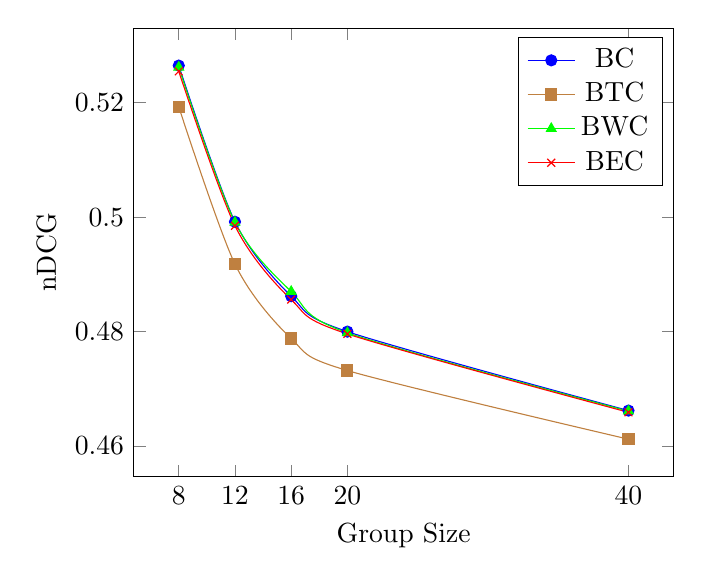
\begin{tikzpicture}
\begin{axis}[
	xlabel=Group Size,
	ylabel=nDCG,
	xtick = {4,8,12,16,20,40}]
		\addplot[smooth,mark=*,blue] plot coordinates {
		%(4,0.6028)
		(8,0.5265)
		(12,0.4992)
		(16,0.4862)
		(20,0.48)
		(40,0.4662)
	};
	\addlegendentry{BC}
	
	\addplot[smooth,color=brown,mark=square*] plot coordinates {
		%(4,0.5995)
		(8,0.5193)
		(12,0.4918)
		(16,0.4788)
		(20,0.4732)
		(40,0.4612)
	};
	\addlegendentry{BTC}
	
	
	\addplot[smooth,color=green,mark=triangle*] plot coordinates {
		%(4,0.6022)
		(8,0.5262)
		(12,0.4991)
		(16,0.487)
		(20,0.4798)
		(40,0.4661)
	};
	\addlegendentry{BWC}
	
	
	\addplot[smooth,color=red,mark=x] plot coordinates {
		%(4,0.6010)
		(8,0.5255)
		(12,0.4985)
		(16,0.4856)
		(20,0.4796)
		(40,0.4659)
	};
	\addlegendentry{BEC}

\end{axis}
\end{tikzpicture}
\caption{Results using nDCG on BC extensions}\label{fig:appendixndcg}
\end{figure}
\subsubsection{Distance Measures}\label{sec:distance}
Before going through the distance measures, we want to cover some general notations that both methods use. As we work with comparing two top-k lists, which are partial lists, we denote them as $\tau_1$ and $\tau_2$. $\tau_1 (i)$ is the notation for the position of element $i$ in $\tau$. $Z = \tau_1 \cap \tau_2$, $z=|Z|$, $S$ is the set of items in $\tau_1$ but not $\tau_2$ and $T$ is vice versa, and $k$ is the length of the top-k lists.

\adparagraph{Kendall Tau Distance}
The idea of Kendall tau distance(KTD) is to compare two ranked lists based on the order in which the items appear. This basically means that it makes pairwise comparisons of item indexes $\{i,j\}$ where $i < j$, so that if $i$ is before $j$ in $\tau_1$ then this should also be the case in $\tau_2$ in order to get a good score. The score is based on a count of how many times $i$ and $j$ are in reverse order. The equation for KTD for complete lists can be seen in Equation \ref{eq:kendalldistancefinal} where $K_1$ and $K_2$ can be seen in Equation \ref{eq:kendalldistance1} and \ref{eq:kendalldistance2} respectively.

\begin{equation}\label{eq:kendalldistance1}
K_1(\tau_1,\tau_2) = | \{(i,j) | i < j, \tau_1 (i) < \tau_1 (j) \land \tau_2 (i) > \tau_2 (j)\}|
\end{equation}
\begin{equation}\label{eq:kendalldistance2}
K_2(\tau_1,\tau_2) = | \{(i,j) | i < j, \tau_1 (i) > \tau_1 (j) \land \tau_2 (i) < \tau_2 (j) \} |
\end{equation}
\begin{equation}\label{eq:kendalldistancefinal}
K(\tau_1,\tau_2) = K_1(\tau_1,\tau_2) + K_2(\tau_1,\tau_2)
\end{equation}

In order to adjust KTD for partial lists we used the $K_{Haus}$ algorithm proposed by Fagin et al\cite{comparing:topk}. This approach has four different cases.

The first case is when both $i$ and $j$ appear in $\tau_1$ and $\tau_2$. In this case the method utilizes Equation \ref{eq:kendalldistancefinal} but only on the items in the set, $Z$.

The second case is when $i$ and $j$ both appear in $\tau_1$ or $\tau_2$ but only $i$ or $j$ appears in the other. Case two is calculated according this formula $(k-z)(k+z+1)- \sum_{i \in S} \tau_1(i)- \sum_{i \in T} \tau_2(i)$. The formula takes the maximum number of items and subtracts the positions from the list containing the items.\note{Revise this explanation, as it is more complex.}

Third case is when $i$ appears in one list and $j$ in the other. For these cases the distance is measured as $(k-z)^2$, which is the disjunctive union of both lists to the power of 2.

The fourth case is when both $i$ and $j$ appear in one list but not the other. In this case Equation \ref{eq:case4} is used. $p$ in this case is a penalty value between 0 and 1. As the method we use is an average approach this value is naturally 0.5. $p$ is multiplied with the binomial coefficient of the length of different items in the top-k lists.

\begin{equation}\label{eq:case4}
2p\left(\!
    \begin{array}{c}
      k-z \\
      2
    \end{array}
  \!\right)
\end{equation}


Combining these cases into one method, we get the $K_{Haus}$ algorithm which can be seen in Equation \ref{eq:khaus}. 
\footnotesize
\begin{equation}\label{eq:khaus}
K_{Haus}(\tau_1,\tau_2) = \frac{1}{2}(k-z)(5k-z+1)+ \sum_{i,j \in Z} K_{i,j}(\tau_1,\tau_2) + \sum_{i \in S}\tau_1(i) - \sum_{i \in S}\tau_1(i)
\end{equation}
\normalsize

The result of the $K_{Haus}$ is normalized by dividing it by $n(n-n)/2$, which gives an approximation of the average distance between the lists. It is an approximation because in case four, the method assumes that there is an equally large chance of the items being in the correct order. Due to this, the method returns 0.78 if the lists are completely disjoint. If the lists are reverse of each other it scores 1 and 0 if the lists are equal. %For a more detail explanation of $K_{Haus}$ go to Fagin et al\cite{comparing:topk} article.

 
\note{Mention somewhere that the results are averages of all group members and all groups}

\adparagraph{Spearman's Footrule Distance}
Another distance measure we use is the Spearman's Footrule Distance(SFD). SFD finds the exact distance between item $i$ in two different ranked lists containing $i$. The way it finds this item distance is by subtracting the item indexes from each other as can be seen in \ref{eq:sfd}. 

\begin{equation}\label{eq:sfd}
F(\tau_1, \tau_2) = \sum_{i=1}^{k} | \tau_1 (i) - \tau_2 (i) |
\end{equation}

As we work with partial lists we use an alternate version called $F_{Haus}$, see Equation \ref{eq:fhaus}, proposed by Fagin et al\citep{comparing:topk}.
As the lists $\tau_1$ and $\tau_2$ can contain different items, the missing index values for items are replaced by $\ell$ which is some value larger than $k$, as it follows that they would be outside the top-k list. Based on the article by Fargin et al we set $\ell$ to be equal to $(3 * k - z + 1)/2$.

\footnotesize
\begin{equation}\label{eq:fhaus}
F_{Haus}(\tau_1,\tau_2)= (k-z)(3k-z+1)+\sum_{i\in Z} | \tau_1 (i) - \tau_2 (i) | - \sum_{i\in S} \tau_1 (i) - \sum_{i\in Z} \tau_2(i)
\end{equation}
\normalsize
% some items will be missing on the lists. In order to handle this we insert $\ell$ which is equal to $(3 * k - z + 1)/2$ placing the item \note{find reason}.  

In order to normalize we divide the result of Equation \ref{eq:fhaus} by $n^2 /2$ which is the maximum value of the algorithm. Doing so we get a value of 0 if $\tau_1$ and $\tau_2$ are in the same order or 1 if the lists are the reverse of each other or completely disjoint.